\section{Motivation}
\label{sec:Motivation}

\begin{wrapfigure}{r}{0.41\textwidth}
		\centering
		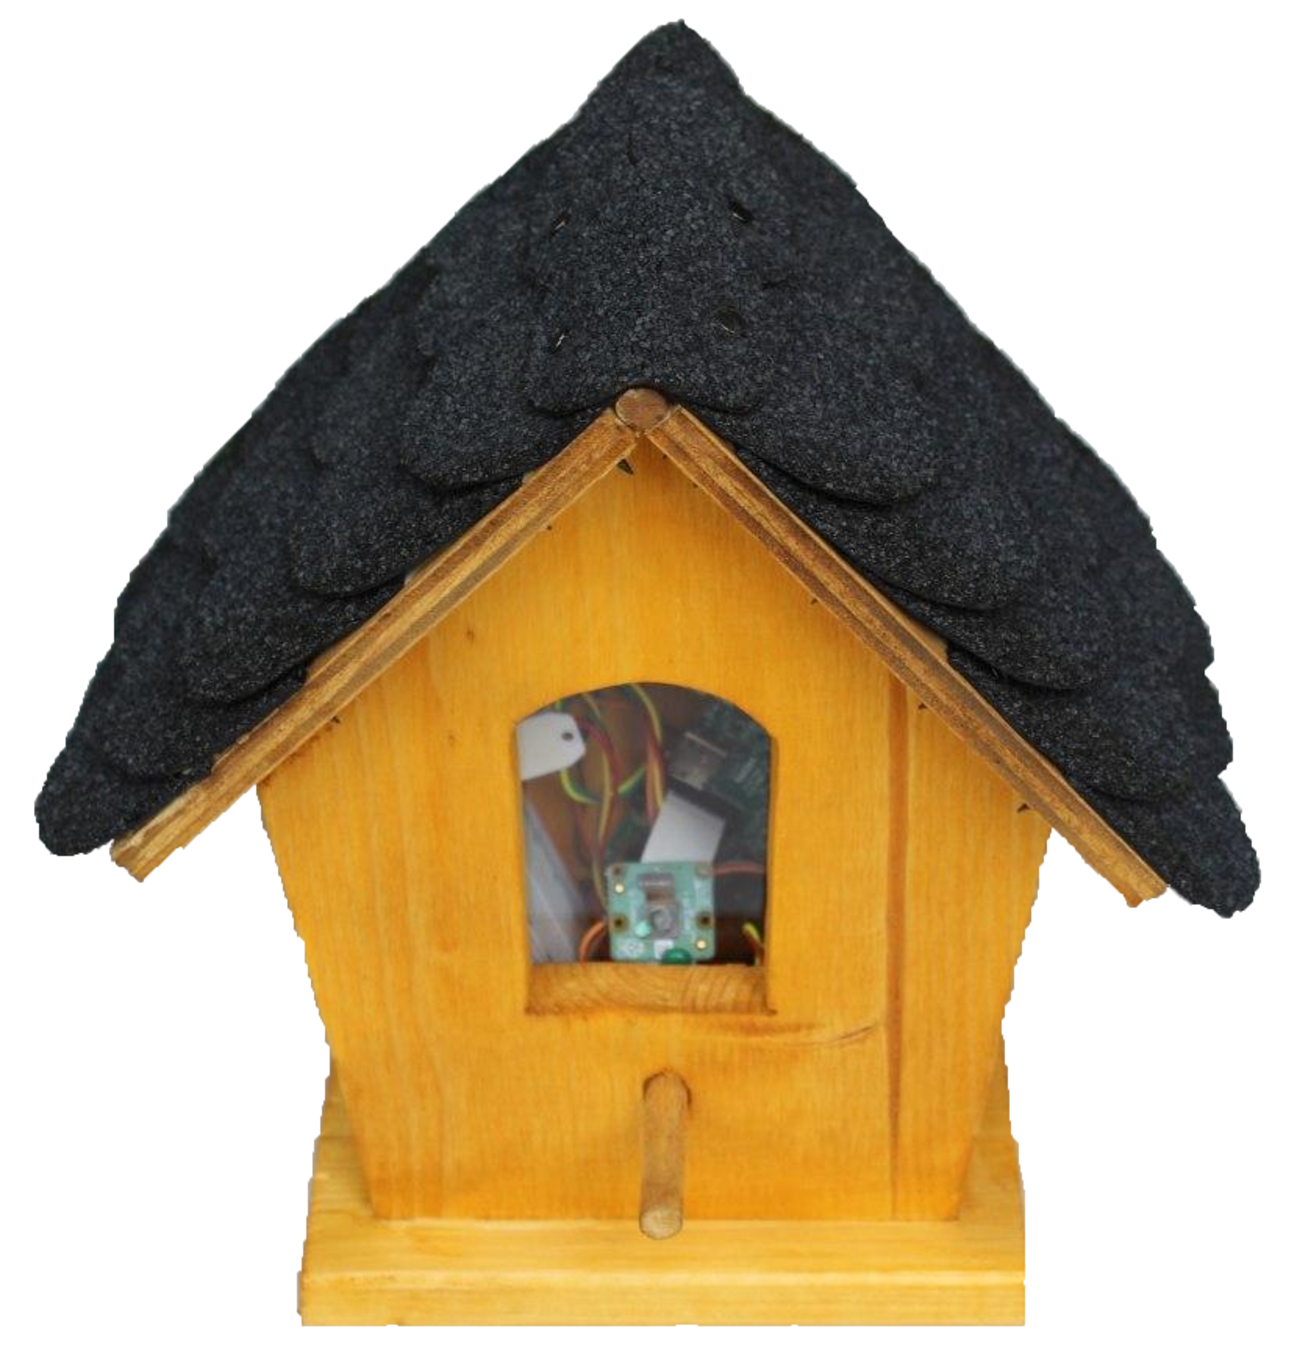
\includegraphics[width=0.4\textwidth]{./pictures/wetterstation.pdf}
		\caption{Wetterstation zur aufnahme der Daten}
		\label{fig:name}
\end{wrapfigure}
Das Weatherpi Projekt entsteht im Rahmen des Physikstudiums.
Es widmet sich der Fragestellung, ob sich mit einfachen mitteln zuverlaessige
Wettervorhersagen erstellen lassen koennen.
Dazu werden locale Daten mittels Sensoren welche an einen einfachen Einplatinencomputer
angeschlossen sind, erhoben.
Diese Daten werden anschliessend auf einen Server hochgeladen welche
flaechendeckende Wettervorhersagen machen soll. \par
Zu den Erhobenen Daten zahlen die Temperatur, der Druck, die Luftfeuchtigkeit
sowie ein Ausschnitt der Wolkendecke.
Um Korrelationen zwischen den einzelenen feature zu entdecken muessen die Daten
bei bekannter Bewoelkung aufgenommen werden.
Desweiteren ist die Wolkendecke auch von notwendigkeit um das Wetterlage genau
zu spezifizieren.  \par
Zur Auswertung der Daten soll eine Live analyse durchgefuehrt werden. 
Diese steht unter der Permisse schnell, genau und recoursenschonend zu seien.
Dazu werden algorithmen des Maschinellen lernenens verwendet. 
Ziel ist es nach der erstellung eines klassifizierten Trainingssatzes, die auf
diesem trainierten Algorithmen bei hinreichend grosser genauigkeit die Klassen
automatisiert zu erkennen.
Wenn das Klassenlabel bekannt ist braucht nicht mehr das Foto zum Server
geschickt werden und der Datentransfer kann reduziert werden. \par
Dazu werden zwei Modelle evaluiert welche auf den beiden Charakeristischen
Eigenschaften des Wolkenspektrums trainiert werde. 
Diese sind einerseits die Formen, sowie das Farbspektrum der Wolken.
Das Farbspektrum laesst sich naive mit einem Random Forrest auswerten zu dessen
staerken eine grosse Generalisierung gehoert. 
Mittels eine Convolutional Neuronal Network (CNN) besteht die Moeglichkeit auf
beiden Information Kanaelen zu trainieren. 
Daher besteht die Hoffnung durch das verwenden einen CNN einen performance Schub
gegenueber den Random Forest zu bekommen. \par
Werden die Wolken entsprechend richtig klassifiziert laesst sich in weiteren
schritten welche nicht Teil des Seminars sind aus der Folge der Wolken der z.B
der Niederschlag berechnen. 
Desweiteren kann die entwicklung der Temperatur aufgrund der Waermespeicherung
und Isolierug von Wolken verbessert werden.

